\chapter[Na\textsuperscript{\scriptsize+}vigating the pressure, sodium fluctuations]{Na\textsuperscript{\scriptsize+}vigating the pressure, sodium fluctuations}

\textit{The team behind this study started as a research team for a three-day datathon event in Lecco, Italy in November 2023 - the GiViTHON - endorsed by the Clinical Data Science of Istituto di Ricerche Farmacologiche Mario Negri IRCCS and Politecnico di Milano. Ten multidisciplinary teams composed of clinicians, nurses, statisticians, and biodata analysts have been challenged to respond to clinical questions and use the subset database for population selection and   key variables extractions.} 

\section {Introduction}
Traumatic brain injury (TBI) is a critical public health issue that frequently leads to long-term disabilities or death. After a TBI, the brain’s ability to regulate itself can be significantly compromised, resulting in a cascade of physiological disruptions. One of the most important of these is impaired autoregulation, which leads to instability in intracranial pressure (ICP) and compromised cerebral perfusion pressure (CPP). Consequently, cerebral blood flow can be reduced, increasing the risk of \textit{secondary brain injury} through ischemia, hypoxia, and further swelling.

The primary aim of treatment is to prevent secondary brain injury. This concept relies on distinguishing between injured brain tissue and salvageable brain tissue. While one portion of the brain may be irreversibly damaged, other areas remain viable but at risk due to inadequate blood flow or rising ICP. Failure to manage these can worsen the damage in these vulnerable regions, ultimately exacerbating the overall brain injury.\\

Dysnatriemias have already been recognized as a marker of severity of disease and related to mortality in the critically ill patient. There is however accumulating evidence that even mild abnormalities of serum sodium could be linked to disease severity and mortality, including changes within the normal range\cite{sakrFluctuationsSerumSodium2013}.

Serum sodium levels are tightly regulated in the human body, but patients with TBI are at higher risk of developing dysnatremias due to various factors such as hyperosmolar therapy, diabetes insipidus and SIADH. Both hypernatremia\cite{maggioreRelationIncidenceHypernatremia2009a}\cite{vedantamMorbidityMortalityAssociated2017a} and hyponatremia \cite{yumotoPrevalenceRiskFactors2015a} have been linked to higher mortality rates and worse outcomes in traumatic brain injury (TBI) patients as well as in aneurysmal subarachnoid hemorrhage (aSAH)\cite{labibSodiumItsImpact2024}\cite{balesEffectHyponatremiaSodium2016}, highlighting the importance of sodium regulation as a key therapeutic goal for individuals with elevated intracranial pressure. While managing serum sodium levels is important, fluctuations in sodium concentration, rather than just the absolute levels, may also  contribute to injury.\\

We therefore investigate the relationship between fluctuations in plasma sodium (deltaNa) and intracranial pressure (deltaICP) to evaluate how sodium variability influences ICP dynamics. Fluctuations are represented as time patients spent with sodium and ICP levels above or below predefined thresholds — referred to as Na Dose and ICP Dose — as well as  fluctuations within physiologic range.\\

\section {Materials and methods}
\subsection{Study population}
The cohort of critically ill patients with TBI was enrolled from a subpart of the Margherita3 electronic health record database - developed by the Italian Group for the Evaluation of Interventions in Intensive Care Medicine\cite{finazziDataCollectionResearch2018} - which contains the comprehensive clinical data of 53640 patients of about 70 italian intensive care units (ICUs). The trauma population in the database consists of 5943 unique IDs. 

The patients were searched based on the International Classification of Diseases (ICD-10) code. The inclusion criteria identified 411  patients who were diagnosed with TBI.

For most of the study variables, the software immediately ran an automatic check for internal consistency, generating queries then sent to physicians for resolution before incorporation of the new data into the database.\\

The inclusion criteria were as follows: (1) age $\geq$ 18 years, (2) TBI as cause of admission, (3) at least one intracranial pressure (ICP) reading, (4) at least one plasma sodium value.
The exclusion criteria were as follows: (1) expected ICU admission patients, (2) ICU admission after elective surgery, (3) ICU stay of less than 72h (20 patients). Patients who died within 72 hours of ICU admission were excluded to focus the analysis on those with potentially salvageable brain injuries.

\subsection{Data Collection}
Baseline parameters within the first day after ICU admission were collected including demographics (e.g., sex, age, weight, admission type), comorbidities (e.g., myocardial infarction, congestive heart failure, chronic pulmonary disease, and renal disease), assessment scale scores (Glasgow Coma Scale, GCS and Acute Physiologic Assessment and Chronic Health Evaluation, APACHE II Scoring System), intracranial pressure and pupil reactivity.

We gathered all serum sodium measurements from ICU admission up to 14 days, or until death, whichever occurred first. Additionally, we recorded data on various therapies, including extraventricular drainage, use of osmotherapy, barbiturate coma, hypothermia, among others. Lastly, we collected outcome data such as 14-day ICU mortality and overall ICU mortality.

The features extracted can be seen in Tables \ref{tab:categorical_features} and \ref{tab:continuous_features}.

\subsection{Generation of Variables and Definitions}

\paragraph{Serum Sodium Concentration on Admission and Na Dose}

Serum sodium concentration on admission was defined as the first available sodium measurement after admission to the Intensive Care Unit (ICU). Hyponatremia and hypernatremia were defined as conditions where at least three consecutive serum sodium values were below 135~mmol/L or above 145~mmol/L, respectively. The \textit{Na Dose} was defined as the area under the curve (AUC) where plasma sodium remains below (for hyponatremia) or above (for hypernatremia) the respective thresholds over time. This metric quantifies the extent and duration of sodium abnormalities, providing a cumulative measure of sodium imbalance.

\paragraph{Glasgow Coma Scale (GCS)}

The Glasgow Coma Scale (GCS) on admission was defined as the first available GCS score after admission to the ICU, with a specific focus on the motor component (GCSm)\cite{kouloulasPrognosticValueTimerelated2013}. Additionally, we evaluated the best GCS scores within the first 24~hours to assess the patient's neurological status over time. 

\paragraph{Intracranial Pressure (ICP) Dose}
The \textit{ICP Dose} is defined as the area under the curve (AUC) where intracranial pressure (ICP) exceeds 22 mmHg, a threshold linked to worse outcomes in traumatic brain injury. It quantifies the combined magnitude and duration of elevated ICP, offering a measure of intracranial hypertension severity.


\paragraph{Analysis of Plasma Sodium and ICP Fluctuations}

We explored the predictive value of the ratio between changes in intracranial pressure (DeltaICP) and plasma sodium (DeltaNa) - expressed as DeltaICP/DeltaNa - considering the dynamic nature of their relative changes over time. 

To achieve this, we first generated continuous curves for both Na and ICP using linear interpolation. For Na, linear interpolation was applied between the first and last available sodium concentration values obtained from ABG samples, generating interpolated values at one-minute intervals across the entire timeframe. The same interpolation process was applied to the ICP data, resulting in a continuous curve of ICP values at one-minute intervals. This step ensures a consistent temporal resolution for both variables, enabling a detailed analysis of their fluctuations.

Using a literature-based timeframe[37][30] to estimate the delay between changes in plasma sodium and corresponding changes in ICP, we applied a grid search method based on Granger causality\footnote{Granger causality is a statistical method that tests whether past values of one variable can predict future values of another. If one variable improves the prediction of another, it is said to “Granger- cause” the other.} to identify the best-fitting time difference. This optimal value ($\tau$) was then used to shift the ICP curve relative to the sodium curve. DeltaNa and DeltaICP were defined, corrispectively, as the time differences between consecutive values for both Na and ICP, based on the time-lag between the Na curve and the ICP curve (represented by the previously defined $\tau$).
%A further grid search was performed using multiple and submultiple values of the delta-time to identify the best-fitting one.

The concept of $\tau$ is crucial in this context as it represents the time delay between a change in Na (cause) and its resulting effect on ICP (effect). For instance, if we consider time points $T_0$ and $T_1$ for Na, and the same time points for ICP, it would be incorrect to directly correlate these changes without accounting for the time it takes for a change in Na to affect ICP. 


%To determine the optimal $\tau$, we initially employed Granger causality analysis, a statistical method that assesses whether past values of one time series can predict future values of another. This step served to confirm the well-established directional relationship where changes in Na levels influence subsequent changes in ICP (Na $\rightarrow$ ICP) as documented in the literature. However, while Granger causality validated the direction of influence, it \textit{did not provide a statistically significant universal value for} $\tau$ across the patient population. This finding indicated that a fixed $\tau$ could not adequately describe the relationship for all patients.

%Given this limitation, we adopted an empirical approach using a grid search to identify the optimal $\tau$ for each patient. The grid search involved testing various $\tau$ values within a plausible range based on clinical knowledge and previous studies \textcolor{blue}{Ti va se mettiamo proprio i valori?} For each $\tau$ value tested, the Na and ICP curves were aligned accordingly, and we evaluated which alignment produced a dataset that resulted in the best performance of downstream machine learning (ML) models. This data-driven method allowed us to select the most appropriate $\tau$ for each patient, taking into account individual variability in the time delay between changes in Na and their effects on ICP.

By selecting the $\tau$ that maximized the predictive accuracy of the ML models, we ensured that the time-series alignment was optimized for subsequent analysis. This iterative optimization provided a tailored approach for each patient, enhancing the reliability of the calculated DeltaICP/DeltaNa values and their use in predicting patient outcomes.

%In summary, the procedure involved generating interpolated time-series data for Na and ICP, confirming the Na $\rightarrow$ ICP relationship with Granger causality, and using a grid search approach to empirically determine the optimal $\tau$ for aligning these curves. By validating that \(\frac{\Delta \text{ICP}}{\Delta \text{Na}}\) contains relevant and essential information for predicting outcomes, we emphasize its potential value for informing ICU treatment decisions.

Once the curves were aligned using the optimal time delay ($tau$), it was necessary to select a time interval, referred to as "delta time," for calculating the differences between consecutive samples in both the sodium (Na) and intracranial pressure (ICP) curves. The delta time represents the time interval between each sample point and its preceding one, which determines the granularity of the observed changes (DeltaNa and DeltaICP). 
A further grid search was performed for the delta-time to identify the best-fitting one, starting from multiple or submultiple of the tau value.

\subsection{Therapy Intensity Level}
We  divided the patients into three subgroups based on their maximum TIL (Therapy Intensity Level) reached during the observation window. The TILs were simplified from the stepwise therapy and therapeutic TILs proposed in other studies. A more detailed categorisation wasn’t possible due to the absence of certain key variables in the dataset (such as decompressive craniectomy and hypertonic solution therapy). See Table \ref{tabTIL}

\begin{table}[h!]
    \centering
    \renewcommand{\arraystretch}{1.5} % Adjust the row height
    \begin{adjustbox}{width=0.8\textwidth}
    \begin{tabular}{|>{\raggedright\arraybackslash}p{4cm}|>{\raggedright\arraybackslash}p{4cm}|>{\raggedright\arraybackslash}p{10cm}|}
        \hline
        \textbf{Categorized TIL} & \textbf{TIL SCALE} & \textbf{DESCRIPTION} \\
        \hline
        \multirow{2}{*}{\textbf{TIL 1}} 
        & \textbf{No specific therapy} & No specific ICP directed therapy \\
        \cline{2-3}
        & \textbf{Basic} 
        & - Sedation for ventilator/endotracheal tube tolerance* \newline 
        - Volume/vasopressors for non-cerebral nervous system cause (e.g., sepsis, myocardial injury)** \newline 
        - Head-up positioning (ventilator bundle) \newline 
        - Normocapnia (partial pressure of carbon dioxide PaCO$_2$ $\geq$ 40 mmHg) \\
        \hline
        \multirow{2}{*}{\textbf{TIL 2-3}} 
        & \textbf{Mild} 
        & - Higher levels of sedation* \newline 
        - Vasopressors/volume for cerebral perfusion pressure (CPP) support** \newline 
        - Low dose osmotic therapy*** \newline 
        - Mild hypocapnia (PaCO$_2$ 35-40 mmHg) \newline 
        - Cerebrospinal fluid (CSF) drainage < 120 ml/day (<5 ml/hour) \\
        \cline{2-3}
        & \textbf{Moderate} 
        & - Higher doses of osmotic therapy*** \newline 
        - Moderate hypocapnia (PaCO$_2$ 30-35 mmHg) \newline 
        - Mild hypothermia ($T>35^\circ\text{C}$)) \newline 
        - CSF drainage $\geq$ 120 ml/day (>5 ml/hour) \\
        \hline
        \textbf{Extreme TIL (eTIL)} 
        & \textbf{Extreme} 
        & - Profound hypocapnia (PaCO$_2$ <30 mmHg) \newline 
        - Extreme hypothermia ($T<35^\circ\text{C}$) \newline 
        - Extreme suppression for ICP control \newline 
        - \st{Secondary decompression (surgery after 24h)} \\
        \hline
    \end{tabular}
    \end{adjustbox}
    \caption{Therapy Intensity Levels (TIL) scale. \footnotesize{Adapted from Robba et. al\cite{robbaTreatmentsIntracranialHypertension2023a}}}
    \small{\flushleft{No information about secondary decompression is available in the database\\$^*$ not possible to differentiate the target of sedation \\$^{**}$ not possible to differentiate the target of vasopressor therapy\\$^{***}$ about osmotic therapy, no information about the dose was available}
    \label{tabTIL}
\end{table}

\subsection{Outcome definition}
The main purpose of this study was to explore the relationship between plasma sodium and intracranial pressure on the outcome of a patient. 

For the machine learning development, a binary outcome has been defined: \textit{alive at 14 days} or \textit{not alive at 14 days}.

Then, in the subgroup analysis, we tried refining the outcome in three subclasses (alive with GCS>8, alive with GCS<8 and death) to grossly explore the neurologic status at 14 days. Both Glasgow Outcome Coma Scale and survival status at discharge were not available in the dataset.

\subsection{Machine learning models development}
In this section the predictive capabilities of different machine learning algorithms (ML models) have being tested on our dataset.

In particularly, the outcome at 14 days (target variable) was considered.
This outcome is binary, expressed as \textit{alive at 14 days} or \textit{not alive at 14 days}.

For each specific binary classification task, to gain as much as possible predictive capabilities, we tested different pipelines using as evaluation metrics the accuracy and the AUC-ROC.
Each pipeline is composed by a scaler\footnote{preprocessing tool in machine learning used to standardize or normalize feature values to ensure that each feature contributes equally to the model by bringing all values into a comparable range}, a feature selection method\footnote {technique used to identify and select the most relevant features (variables) from a dataset with the the highest predictive power to improve performance by reducing noise and avoiding overfitting.} and a machine learning model.
\begin{itemize}
	\item The base model (\textit{Model 1}) has been developed and trained starting from patient demographics and clinical features available comprehensive of summary statics of sodium trends. 
\end{itemize}

Above this base model further features where added, in order:

\begin{itemize}
	\item \textit {Model 2} accounts for the cumulative effect of ICP Dose and Na Dose. As middle step,  both ICP Dose and Na Dose were evaluated individually and then added together.
	\item The third model (\textit{Model 3}) explores the effects of the DeltaICP/DeltaNa informations over the base model. The DeltaICP/DeltaNa features where extracted as outlined in paragraph 3.2.3. 
\end{itemize}

\section {Results}
\subsection{Patient Demographics and Clinical Features}
In this section we present the descriptive characteristics of our population, divided into  categorical variables and numerical (continuous) variables.

\begin{table}[h!]
	\centering
	\small % Reduce font size
	\begin{tabular}{lll}
		\hline
		\textbf{Feature} & \textbf{Category} & \textbf{Count\_n (\%)} \\
		\hline
		SEX & M & 321 (78.10\%) \\
		%SEX & F & 90 (21.90\%) \\
		TYPE & Chirurgico d’urgenza & 229 (55.72\%) \\
		TYPE & Medico & 182 (44.28\%) \\
		OUTCOME & alive at 14 days & 357 (86.86\%) \\
		%dividere tra alive GCS>8, alive GCS<=8 e death 
		% GCS & > 8 & xx (xx\%) \\ 
		% GCS & =< 8 & 54 (13.14\%) \\
		PUPIL & anisocorìa & 217 (52.80\%) \\
		%PUPIL & False & 194 (47.20\%) \\
		%ICPm & True & 372 (90.51\%) \\
		%ICPm & False & 39 (9.49\%) \\
		%ICPm non ho proprio capito cosa sia...
		Hypernatremia & True & 259 (63.02\%) \\ 
		%Hypernatremia & False & 152 (36.98\%) \\
		Hyponatremia & True & 154 (37.47\%) \\
		%Hyponatremia & False & 257 (62.53\%) \\
		\hline
	\end{tabular}
	\caption{Categorical Feature Statistics}
	\label{tab:categorical_features}
\end{table}

\begin{table}[h!]
	\centering
	\tiny % Reduce font size
	\begin{tabular}{lcc}
		\hline
		\textbf{Feature} & \textbf{Mean (unit)} & \textbf{{Range} {[mean-std, mean+std]} {(unit)}} \\ \hline
		Altezza & 173.24 (cm) & [160.63 - 185.86] (cm) \\
		Peso & 81.53 (kg) & [66.77 - 96.28] (kg) \\
		BMI & 25.46 (kg/m$^2$) & [21.31 - 29.61] (kg/m$^2$) \\
		Best GCS during first 24h hours & 6.29 & [3 - 9.84] \\
		%Worst GCS \textcolor{red}{at admission} & 2.41 & 3.14 & [-0.74 - 5.55] \\
		Best GCS Motor response during first 24h hours & 3.05 & [1.13 - 4.97] \\
		%Worst\_GCS\_Motor\_Response & 1.43 & 1.44 & [-0.01 - 2.88] \\
		
		AGE  & 54.83 (years) & [36.75 - 72.90] (years) \\
		APACHE II Score & 27.46& [22.64 - 32.29] \\
		First Sodium Value & 139.59 (mmol/L)  & [135.11 - 144.07] (mmol/L) \\
		Time to Hypernatremia & 48.97 (h)  & [5.95 - 91.99] (h) \\
		Time to Hyponatremia & 55.32 (h)  & [0 - 111.96] (h) \\
		%Na min first 7 days & 135.12 (mmol/L) & 8.76 (mmol/L) & [126.36 - 143.88] (mmol/L) \\
		%Na max first 7 days & 148.33 (mmol/L) & 6.76 (mmol/L) & [141.57 - 155.09] (mmol/L) \\
		%li ricalcolerei come n di pazienti <135 e >145 includendoli in time to hypenatriemia e tyime to hyponatriemia OPPURE LI LASCIAMO aggiungendo comunque i dati di sopra... - vanno SU 14 GIORNI
		Na min first 14 days  & 135.11 (mmol/L)  & [126.35 - 143.87] (mmol/L) \\
		Na max first 14 days  & 148.33 (mmol/L)  & [141.57 - 155.87] (mmol/L) \\
		Na SD first 14 days & 3.53 (mmol/L)  & [1.08 - 5.97] (mmol/L) \\
		%la Na SD altri studi la chiamano Na variability, forse lascerei cosi che genera confusione, va messu anche lui su 14 giorni
		\hline
	\end{tabular}
	\caption{Continuous Feature Statistics. \footnotesize{APACHE: Acute Physiology and Chronic Health Evaluation, BMI: Body Mass Index, GCS: Glasgow Coma Scale, Na max: maximum serum sodium over 14 days, Na min: minimum serum sodium over 14 days, Na SD: standard deviation of plasma sodium over 14 days}}
	\label{tab:continuous_features}
\end{table}

%\subsection{Relationship between serum sodium fluctuations and intracranial pressure}
%\textcolor{red}{VALUTARE INSIEME SE E COME HA SENSO INSERIRE QUESTO PARAGRAFO, IN RIFERIMENTO A QUEL 60\% CIRCA}
\subsection{Relationship of patient descriptives on outcome}
Our reference \textit{Model 1} achieved an AUC of 0,72 considering the patient baseline characteristics (eg. age, sex, weight, body mass index) and comorbidities (comprehensive of APACHE II score) as well as sodium-related summary statistics (min Na, max Na, Na SD, first sodium value, hypernatremia, hyponatremia, time to hypernatremia, time to hyponatremia) or neurologic status descriptive of the first 24hours (ICP monitoring, pupil status, best GCS and best motor GCS).
\begin{figure}[h]
    \centering
    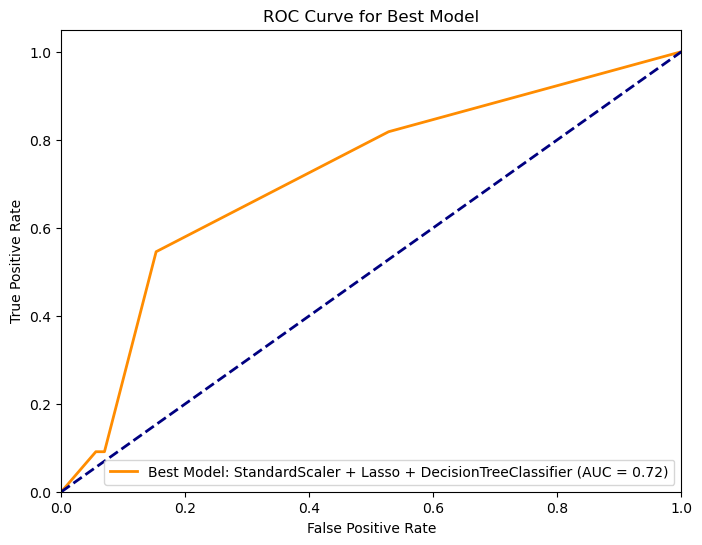
\includegraphics[width=0.6\textwidth]{pictures/fig5_basemodel.png}
    \caption{Reference model} % Add a meaningful caption
    \label{fig:model1} % Add a label for referencing
\end{figure}

\subsection{Relationship Between Na Dose and ICP Dose on outcome}
Our \textit{Model 2} achieved an AUC of 0,85 with a net 18\% improvement over base model. Additionally, over patient descriptives, this model contains informations regarding Na Dose (both above and below thresholds) and ICP Dose.

\begin{figure}[h]
    \centering
    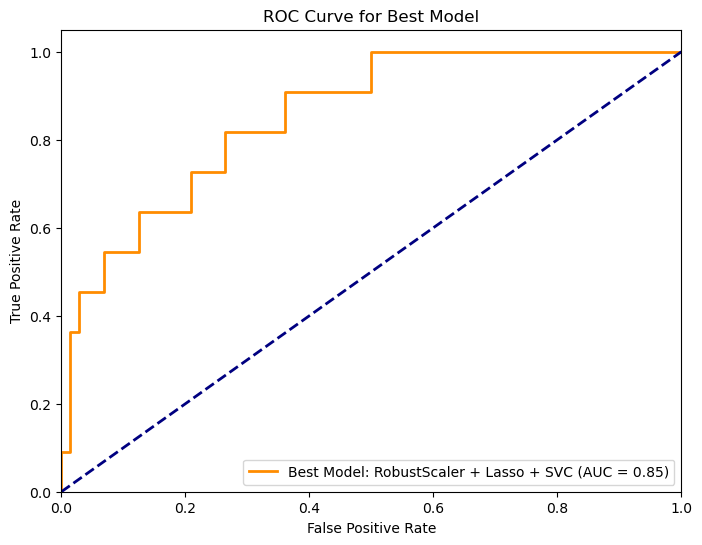
\includegraphics[width=0.6\textwidth]{pictures/fig6_model2.png}
    \caption{Model 2} % Add a meaningful caption
    \label{fig:model2} % Add a label for referencing
\end{figure}

\subsection{Relationship between sodium fluctuations and ICP fluctuations (DeltaICP/DeltaNa) on outcome}
Our last model, \textit{Model 3} was targeting the relative changes between ICP curves and sodium curves over time. It reached an AUC of 0,83 with a 15\% gain  over base model. 

The model 3 is the result of a grid-search testing different tau and delta times, as shown in Figure \ref{fig:model3tau}.

\begin{figure}[h]
    \centering
    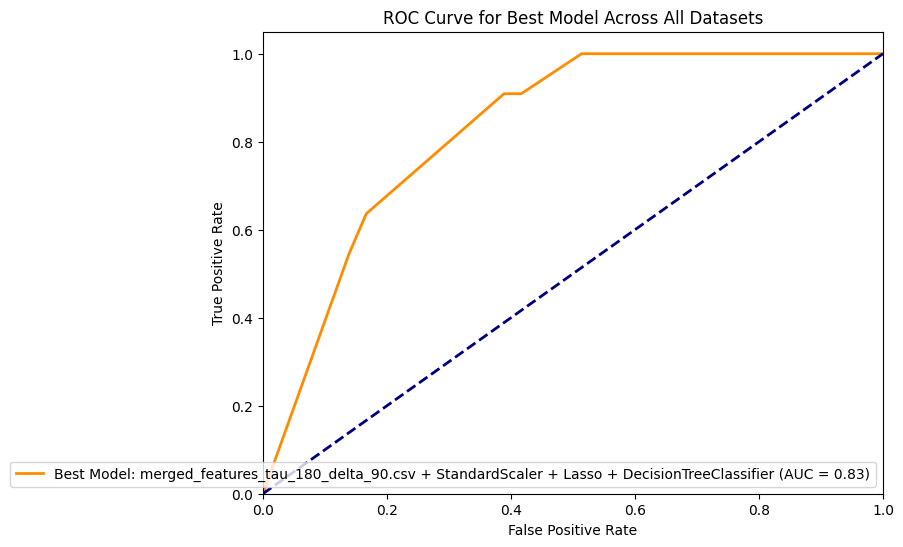
\includegraphics[width=0.8\textwidth]{pictures/fig7_model3.png}
    \caption{Model 3} % Add a meaningful caption
    \label{fig:model3} % Add a label for referencing
\end{figure}
\begin{figure}
	\centering
	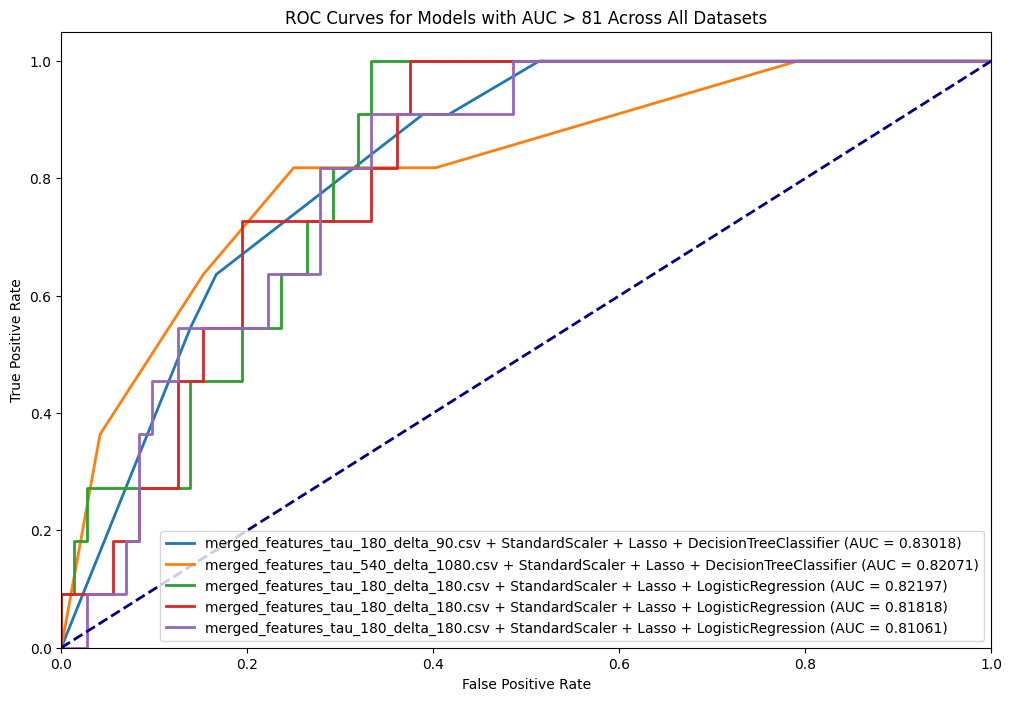
\includegraphics[width=0.8\textwidth]{pictures/fig8_model3tau.png}
	\caption{Testing different combinations with grid search, only AUC>81\% are plotted} % Add a meaningful caption
    \label{fig:model3tau} % Add a label for referencing
\end{figure}


\subsection{Subgroup analysis: outcome}
The following present the relationship between intracranial pressure (ICP) and patient outcomes. Figure \ref{fig:ICPdose_outcome} illustrates the distribution of ICP Dose across different neurological outcomes, categorized by Glasgow Coma Scale (GCS) scores and survival status, showing a trend of increasing ICP burden with worsening outcomes. Figure \ref{fig:ICPfluctuations_outcome} displays the variability in ICP fluctuations across the same outcome groups, highlighting a decrease in fluctuations as the severity of outcomes increases. Lastly, Figure \ref{fig:ICPslope_outcome} presents the linear trend of ICP over time (represented by the ICP signal slope), with a progressive increase in slope correlating with poorer patient outcomes.

\begin{figure}[h!]
    \centering
    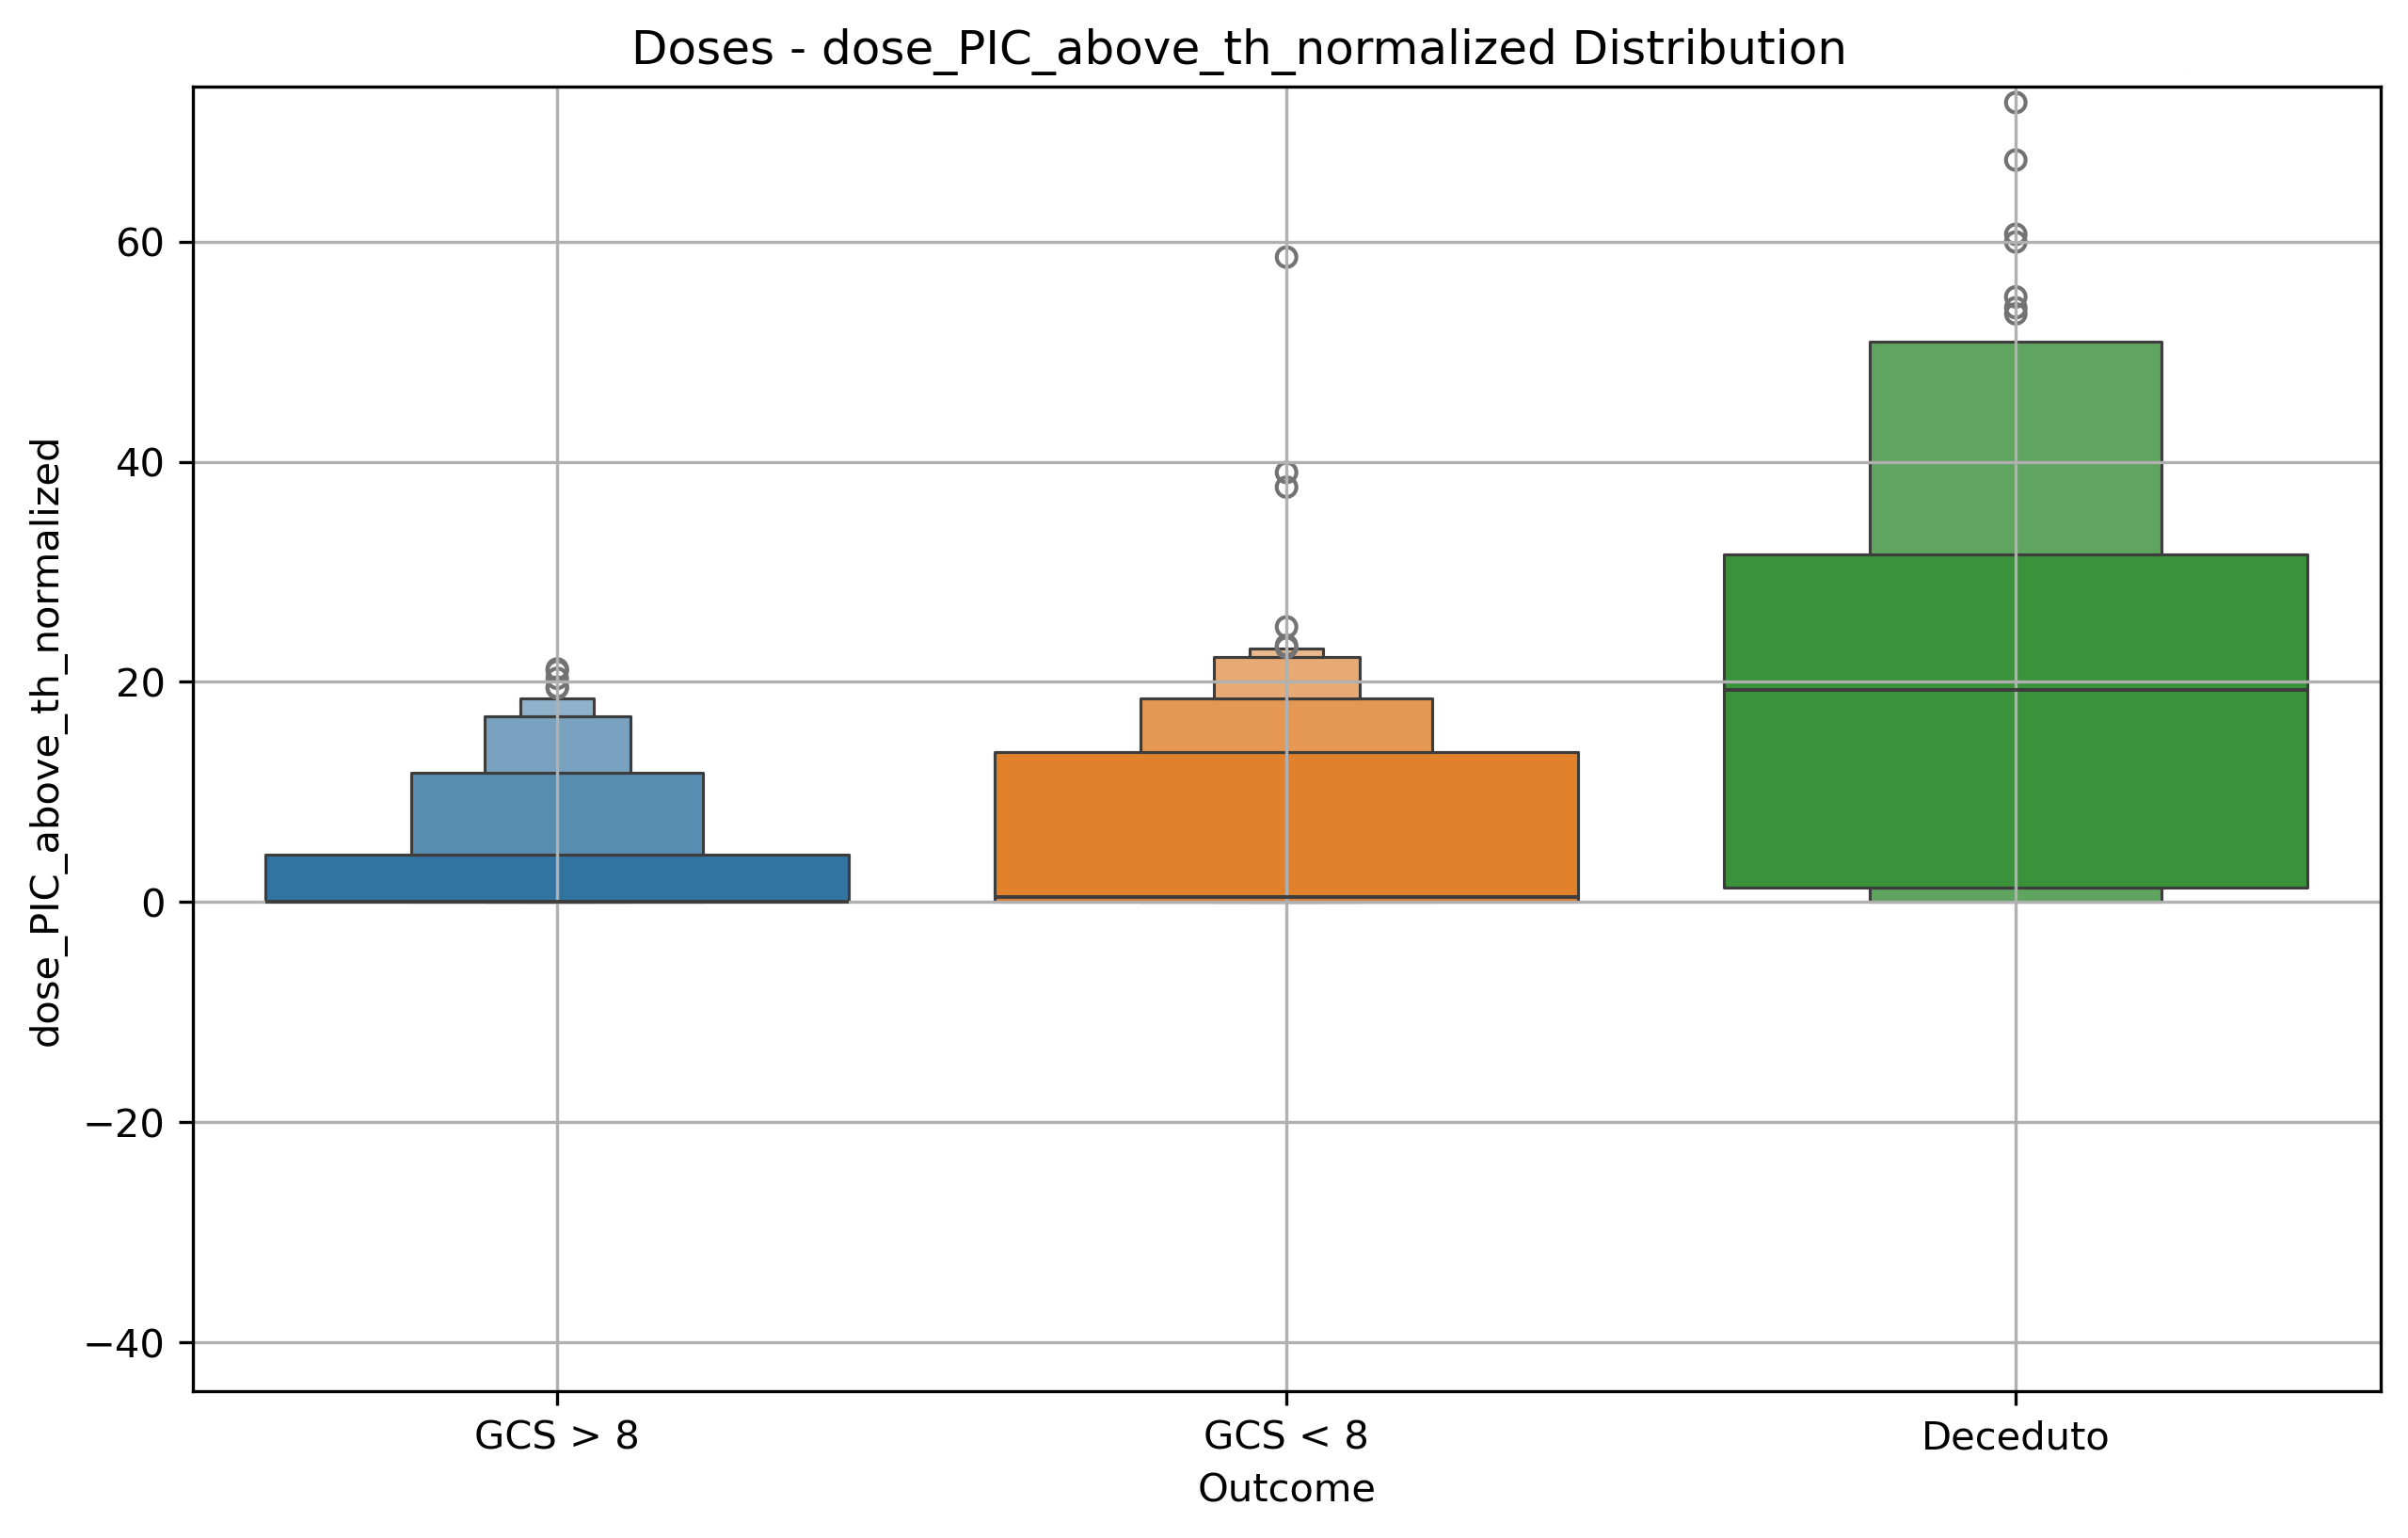
\includegraphics[width=0.8\textwidth]{pictures/fig9_ICPdose.png}
    \caption{ICP Dose and outcome} % Add a meaningful caption
    \label{fig:ICPdose_outcome} % Add a label for referencing
\end{figure}

\begin{figure}[h!]
    \centering
    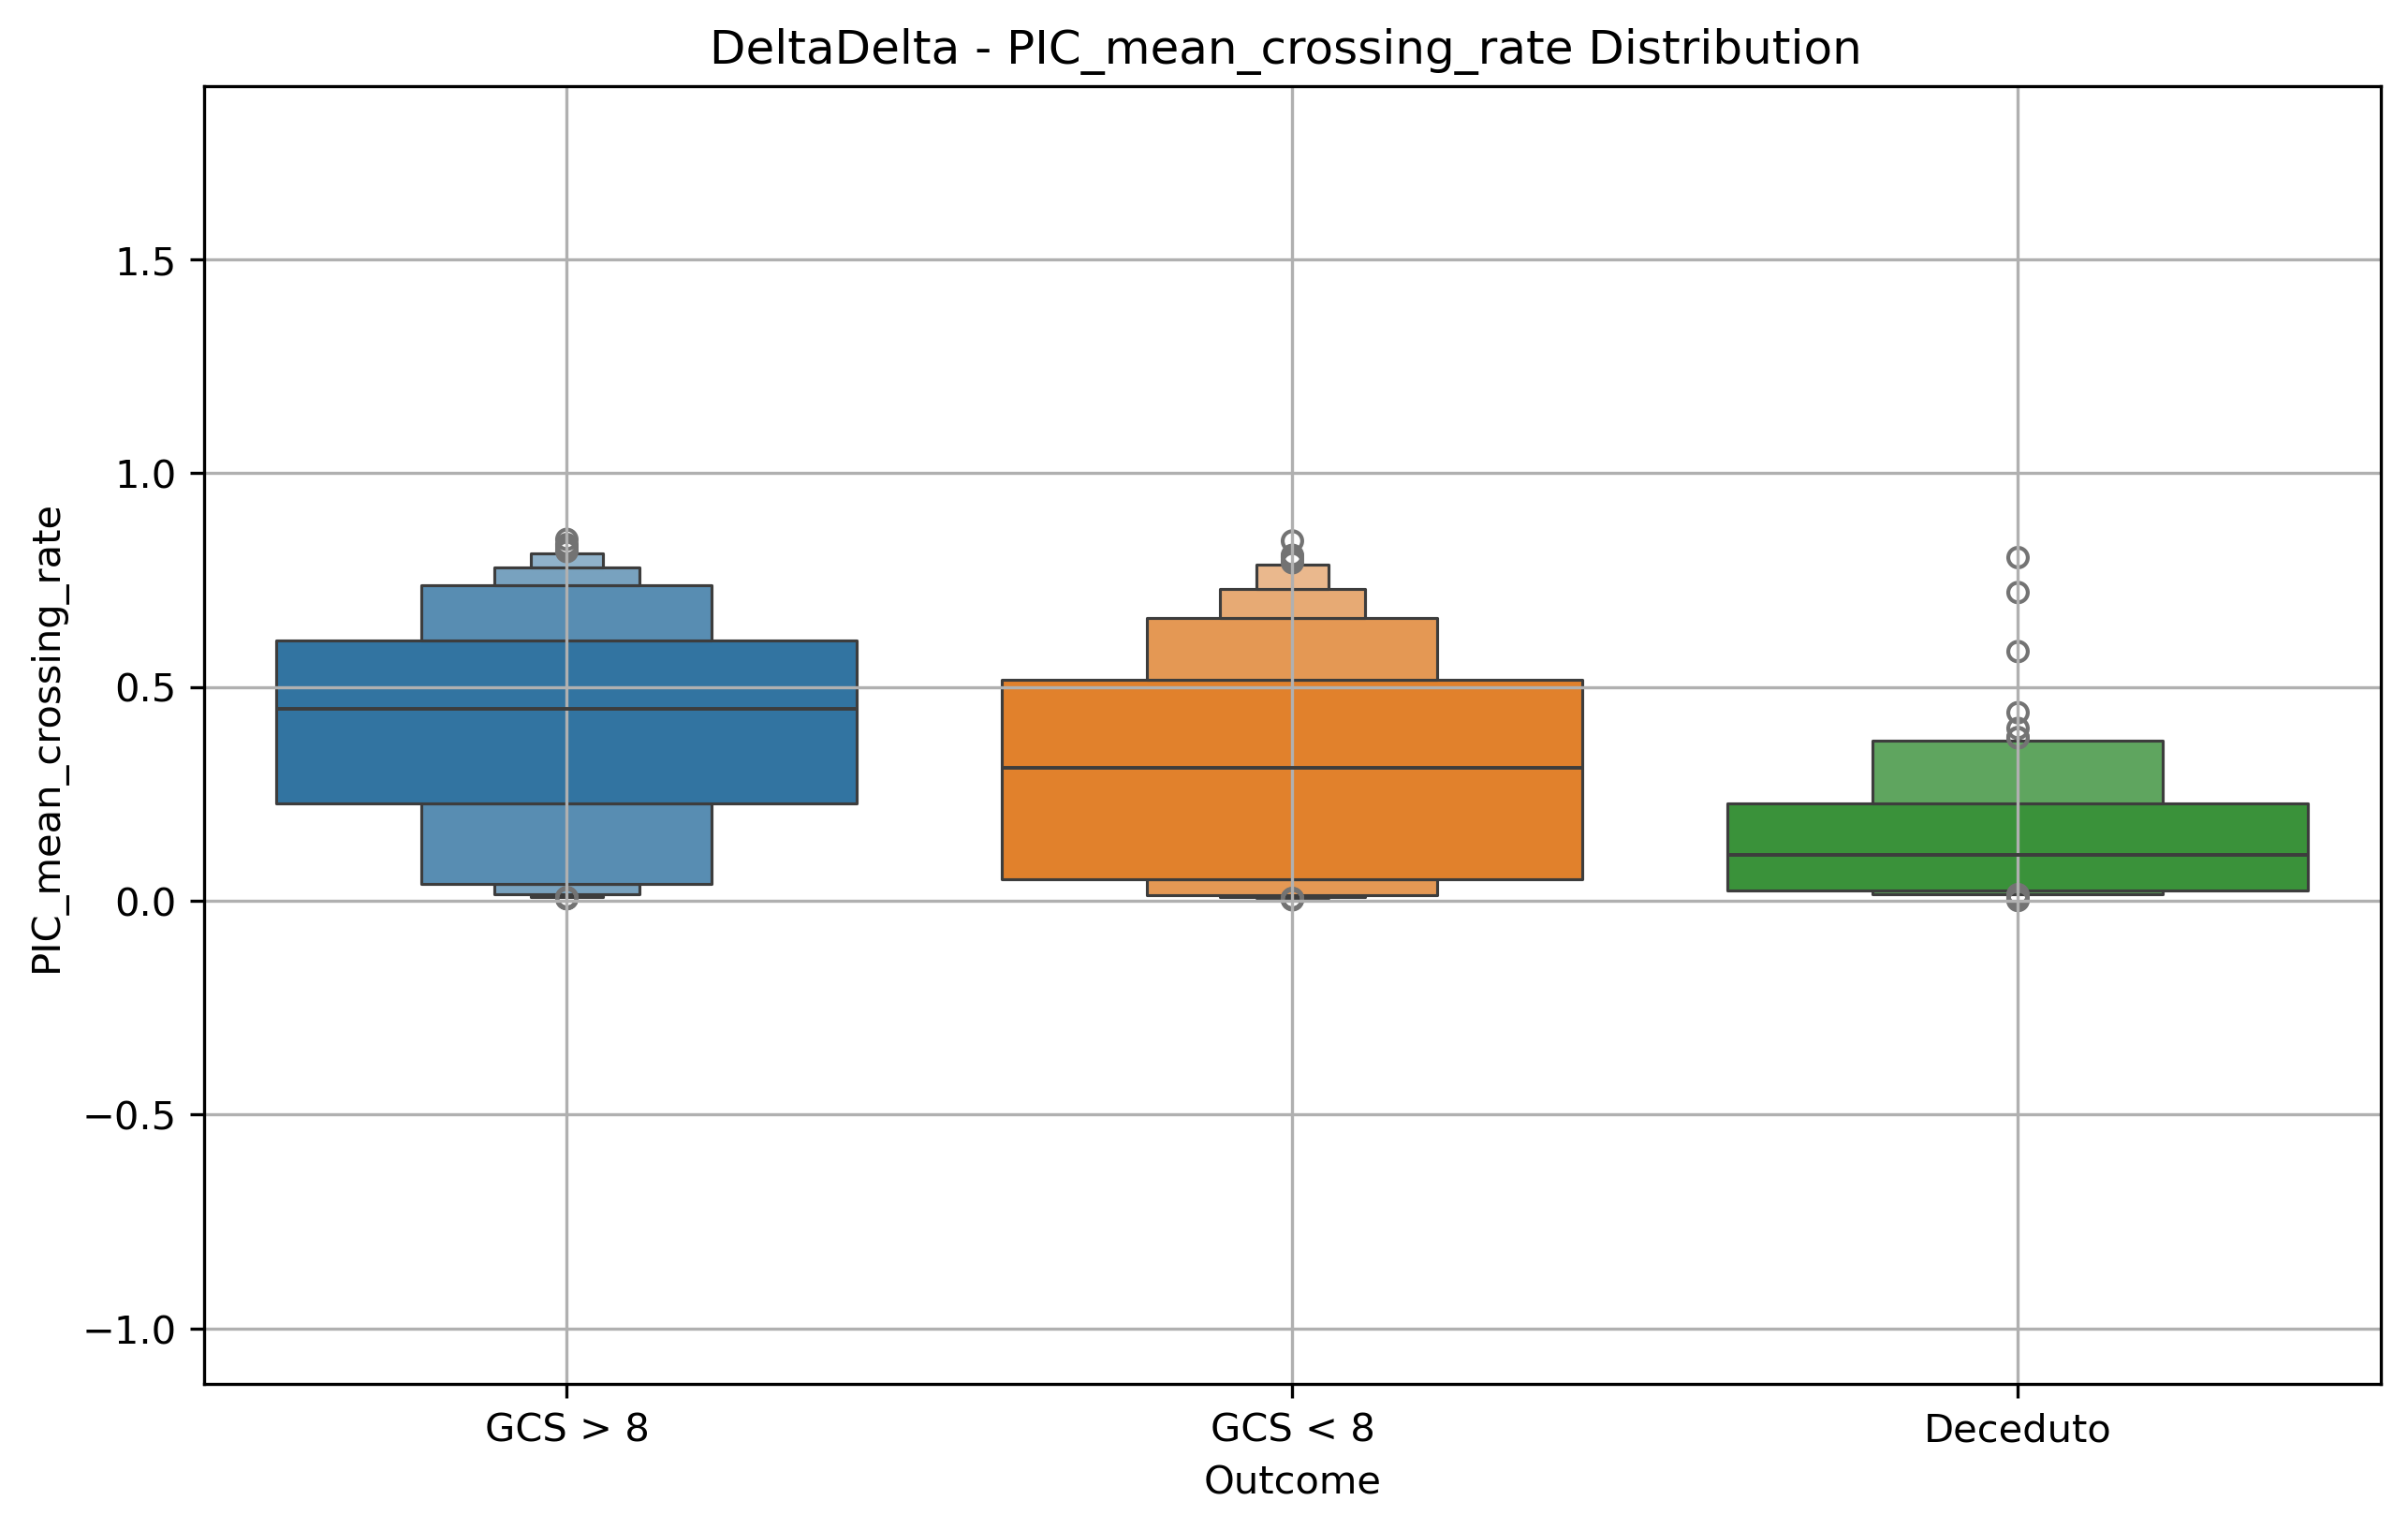
\includegraphics[width=0.8\textwidth]{pictures/fig10_ICPfluctuations.png}
    \caption{ICP fluctuations and outcome} % Add a meaningful caption
    \label{fig:ICPfluctuations_outcome} % Add a label for referencing
\end{figure}

\begin{figure}[h!]
    \centering
    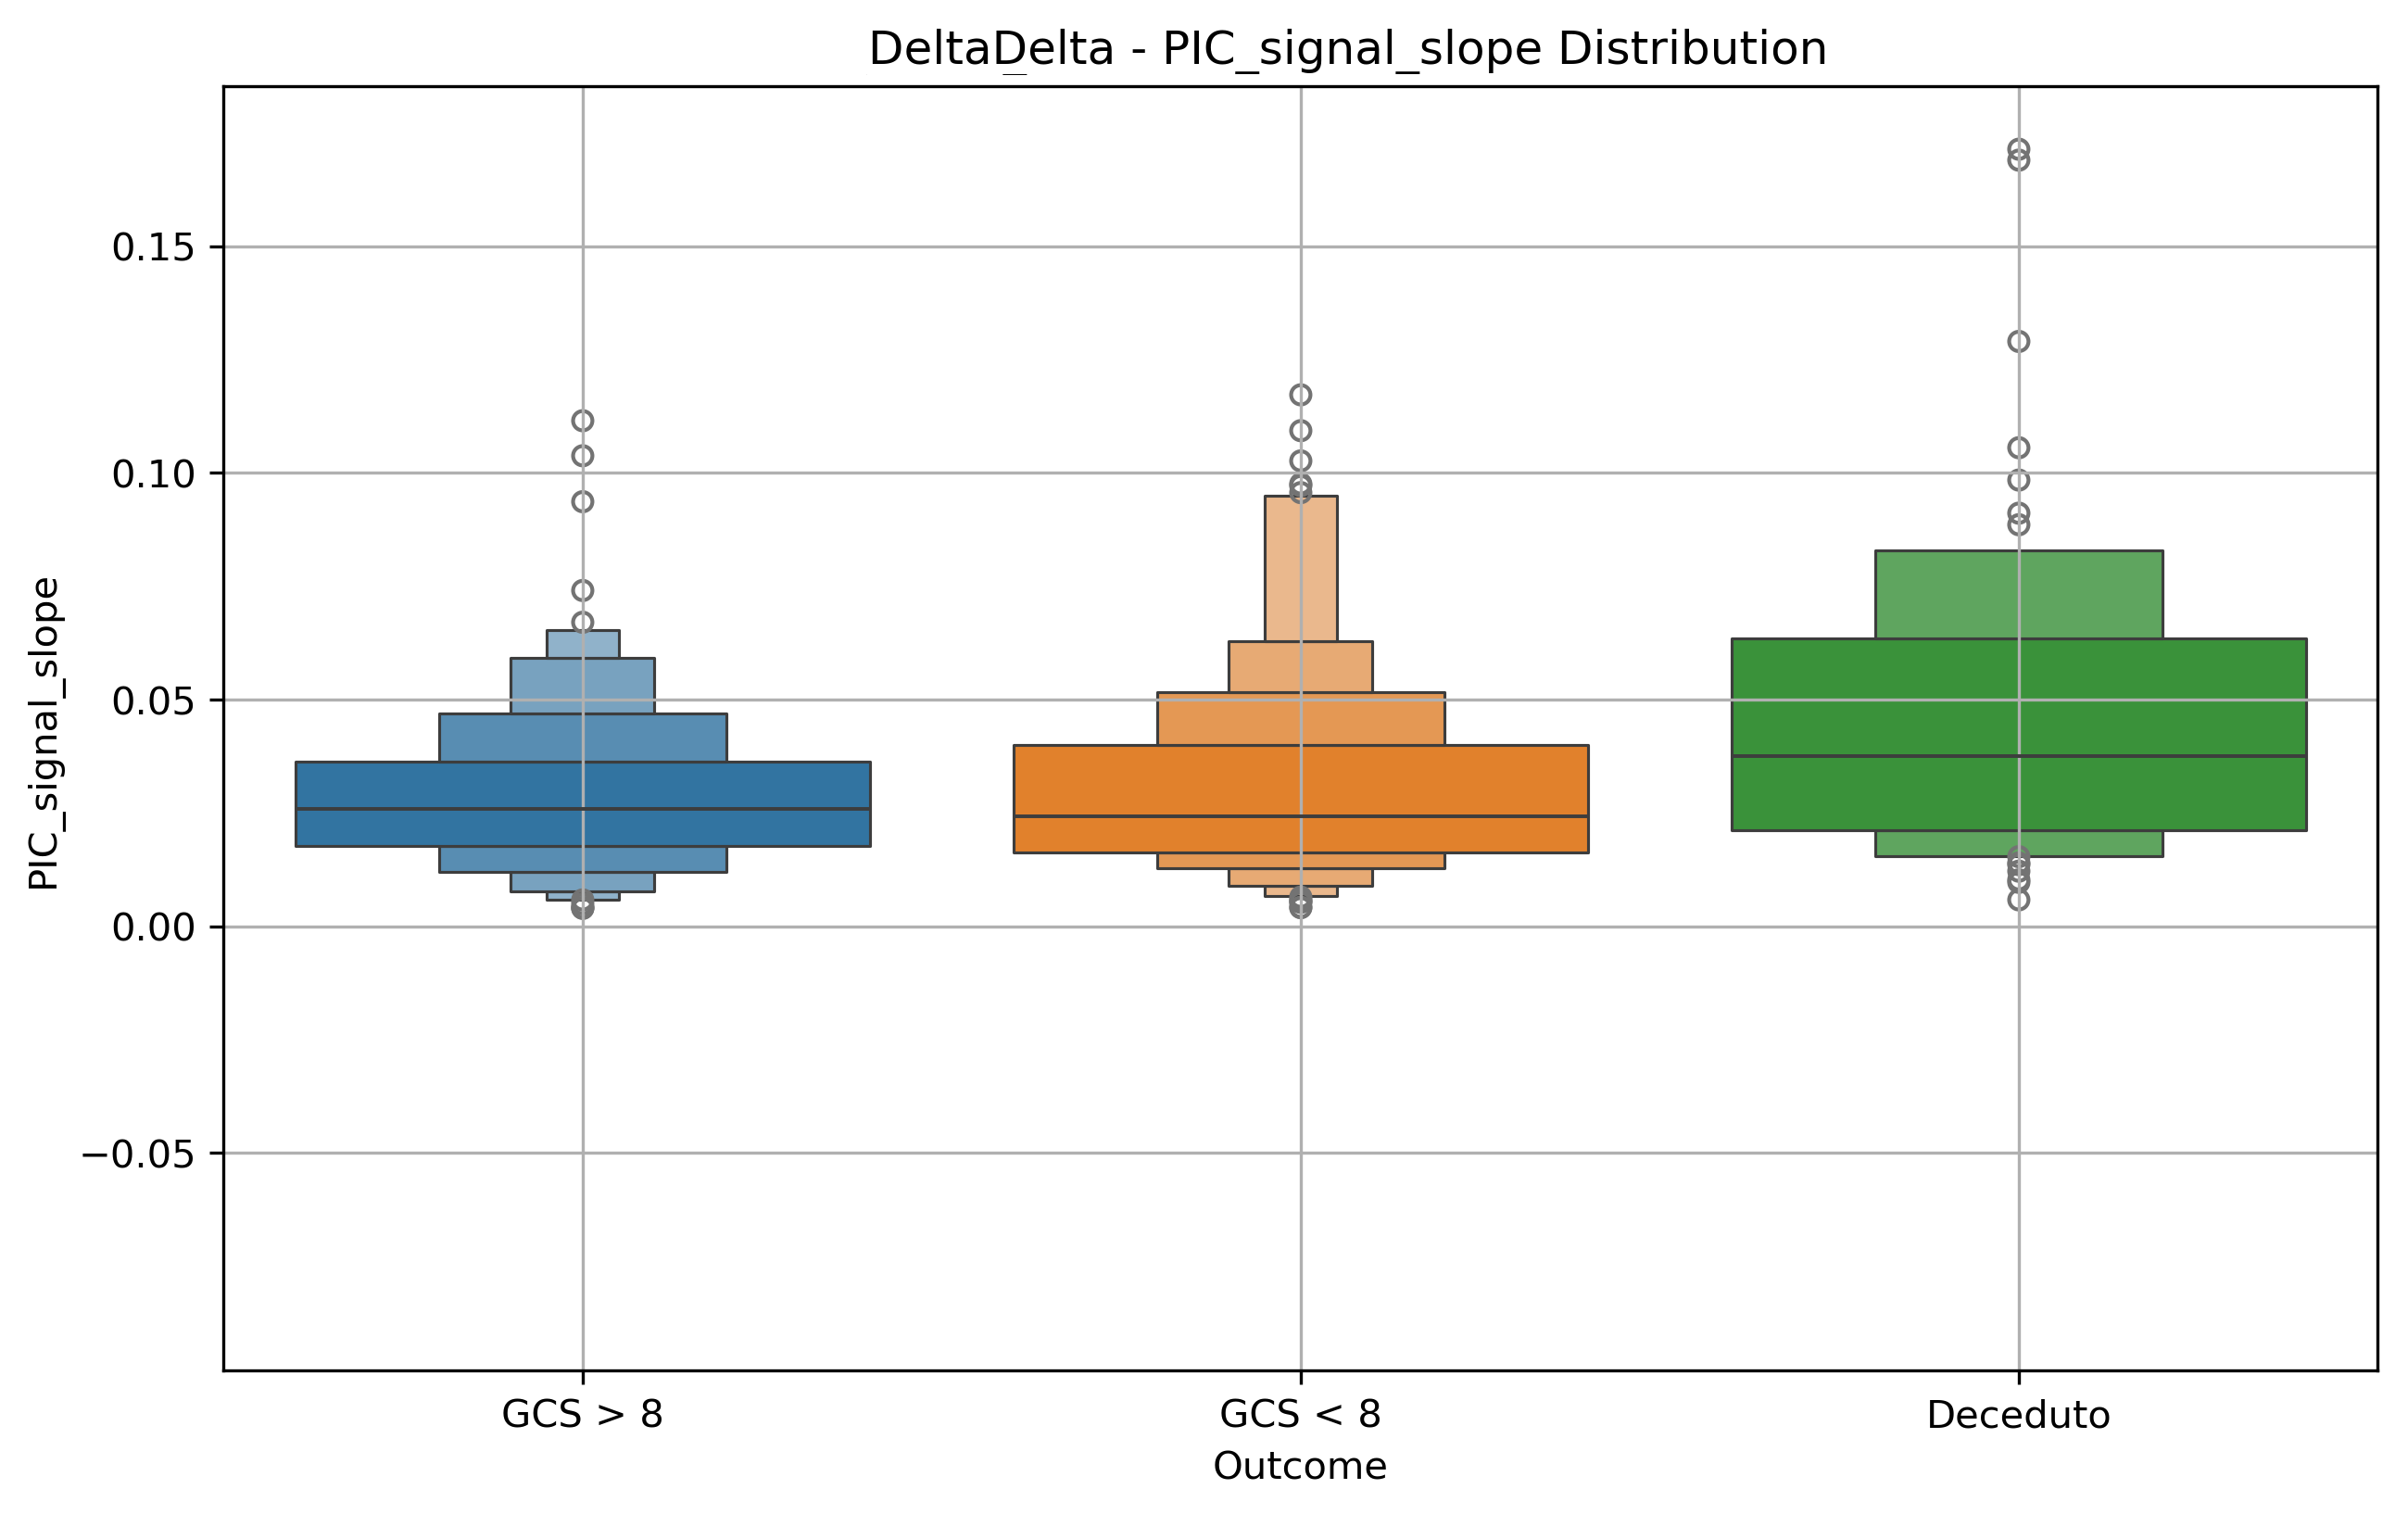
\includegraphics[width=0.8\textwidth]{pictures/fig11_ICPslope.png}
    \caption{ICP linear trend over time and outcome} % Add a meaningful caption
    \label{fig:ICPslope_outcome} % Add a label for referencing
\end{figure}

\subsection{Subgroup analysis: TIL}
The last subgroup analysis focused on ICP and sodium fluctuations across different Therapy Intensity Levels (TILs). 

\begin{table}[h!]
    \centering
    \small % Reduce font size
    \begin{tabular}{lll}
        \hline
        \textbf{TIL class} & \textbf{counts} & \textbf{percentage} \\
        \hline
        eTIL & 51 & 12.4\% \\
        TIL 2-3 & 260 & 63.3\% \\
        TIL 1 & 100 & 24.3\% \\
        \hline
    \end{tabular}
    \caption{TIL Classes.\\\footnotesize{Results aligned with Robba et al. \cite{robbaTreatmentsIntracranialHypertension2023a}}}
    \label{tab:TILclasses}
\end{table}

\begin{figure}[h!]
    \centering
    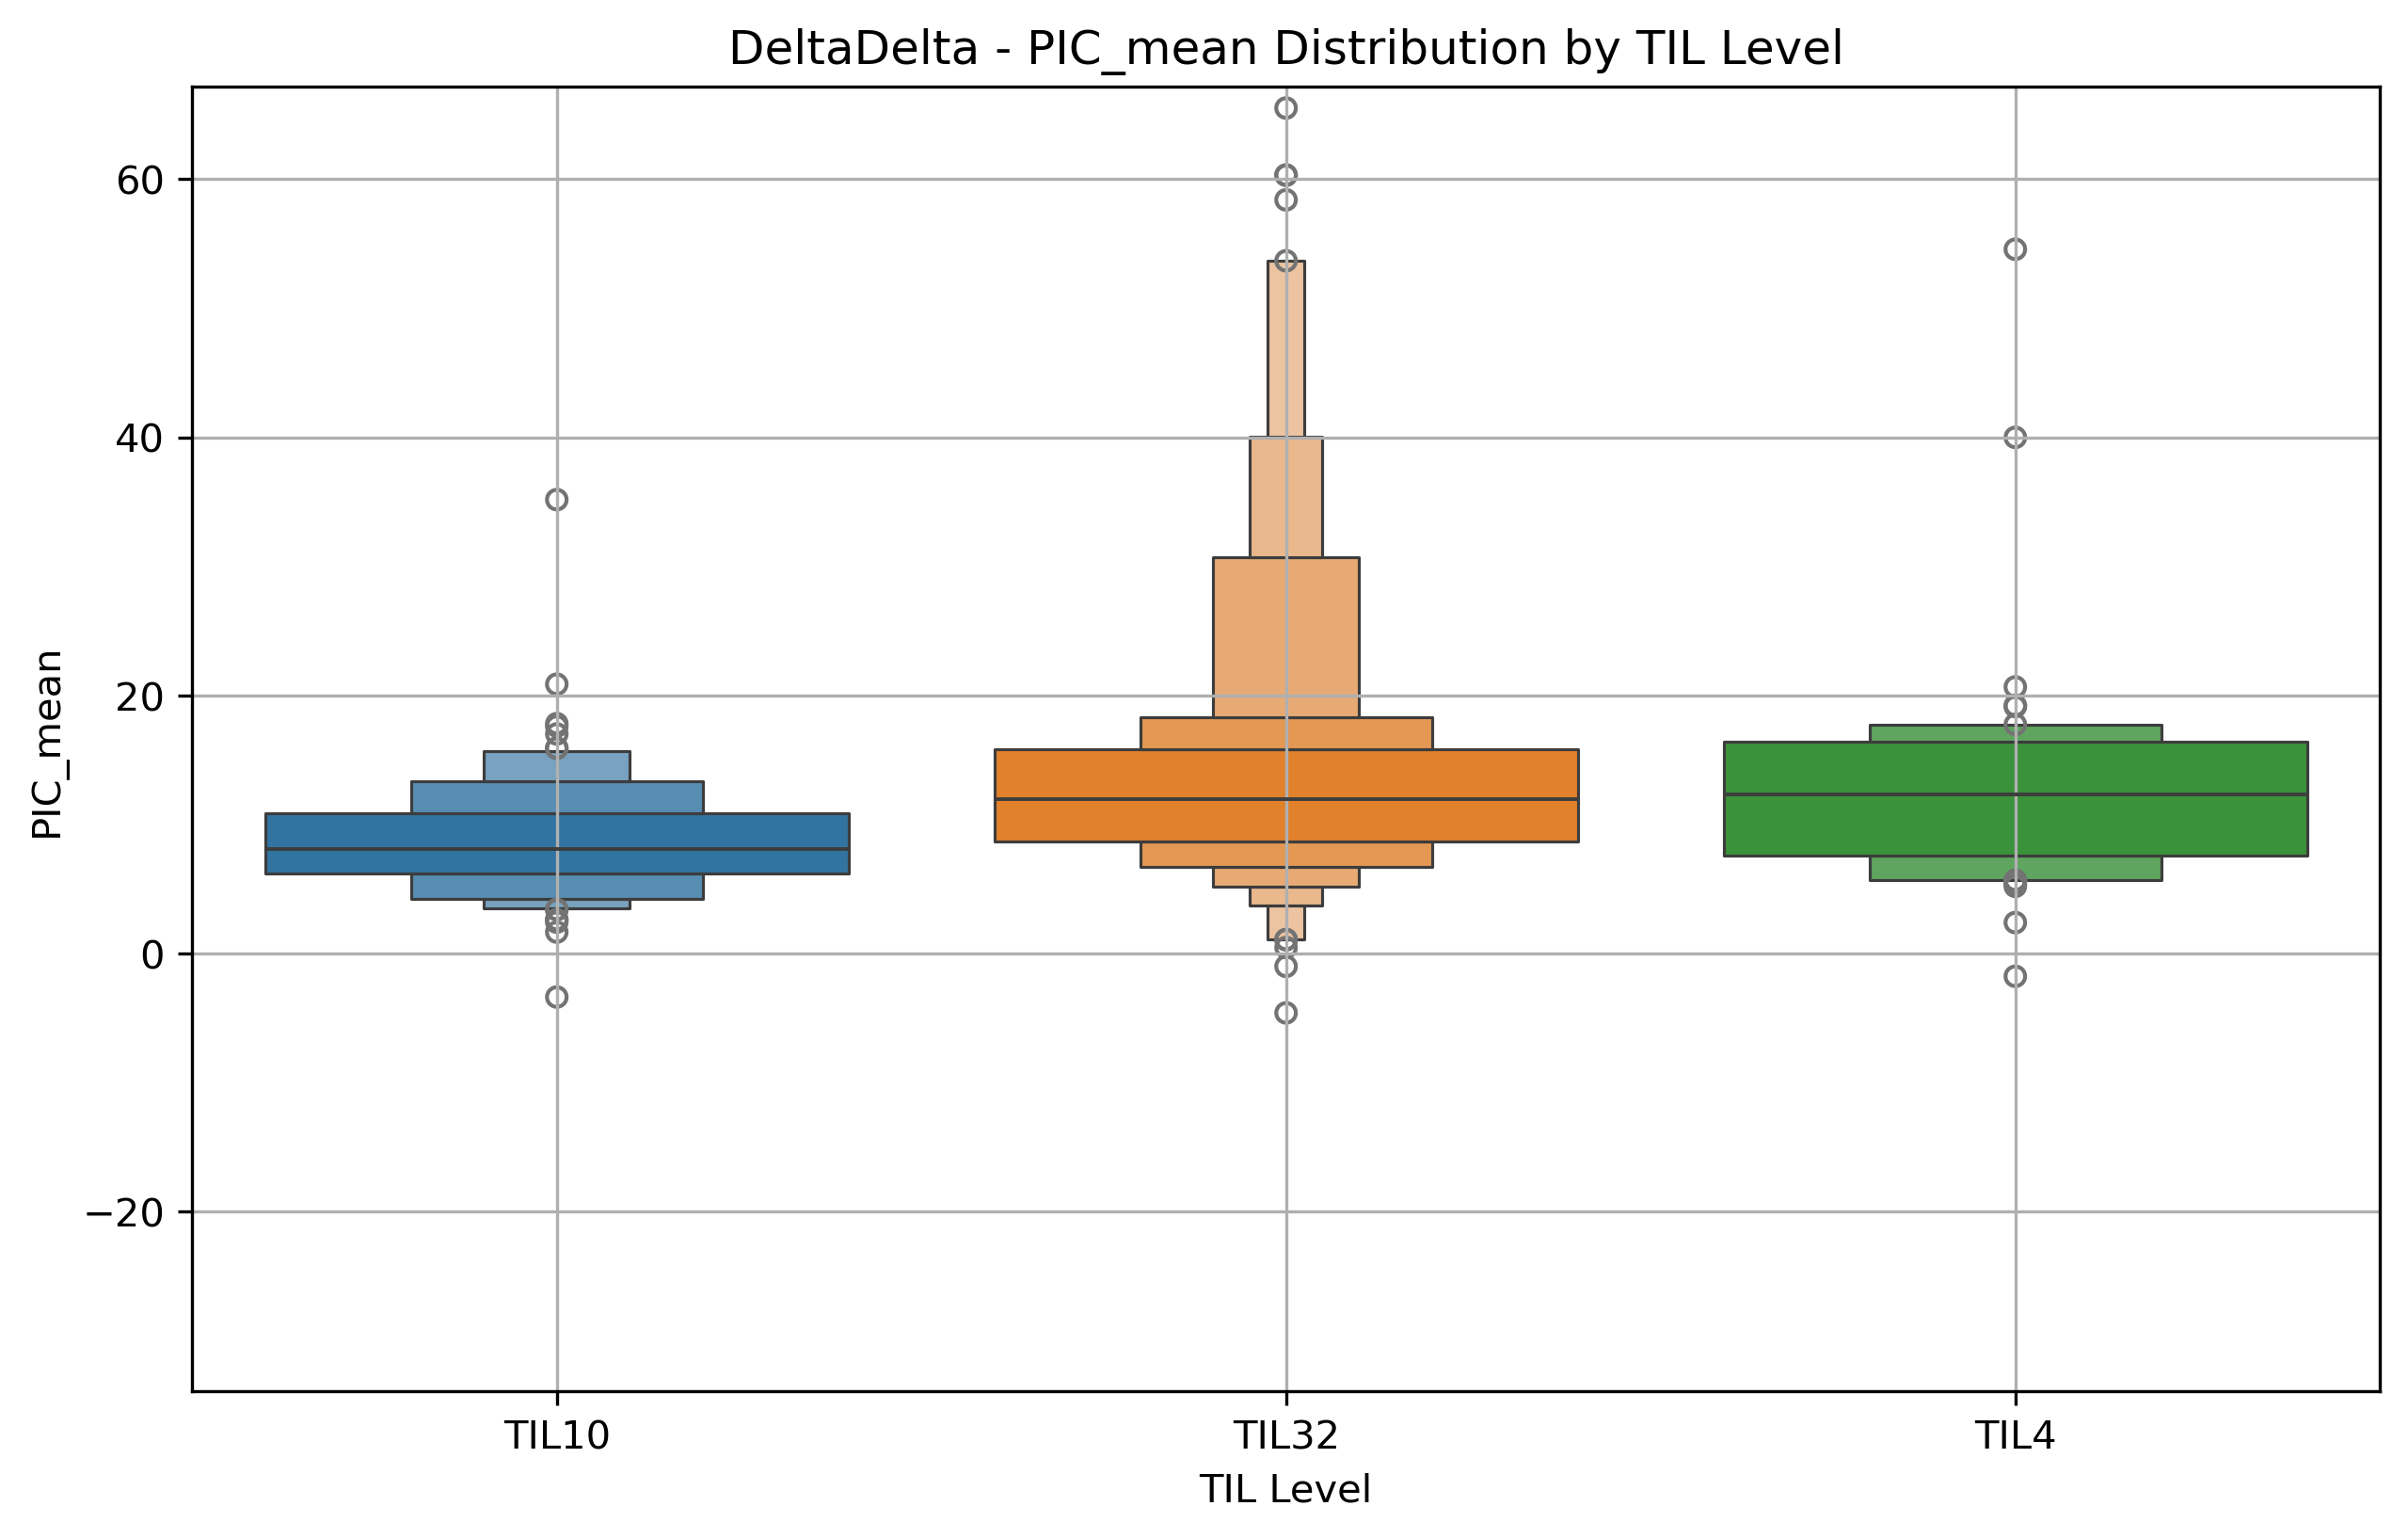
\includegraphics[width=0.8\textwidth]{pictures/fig12_ICPTIL.png}
    \caption{ICP trend in different TIL} % Add a meaningful caption
    \label{fig:ICPTIL} % Add a label for referencing
\end{figure}

\begin{figure}[h!]
    \centering
    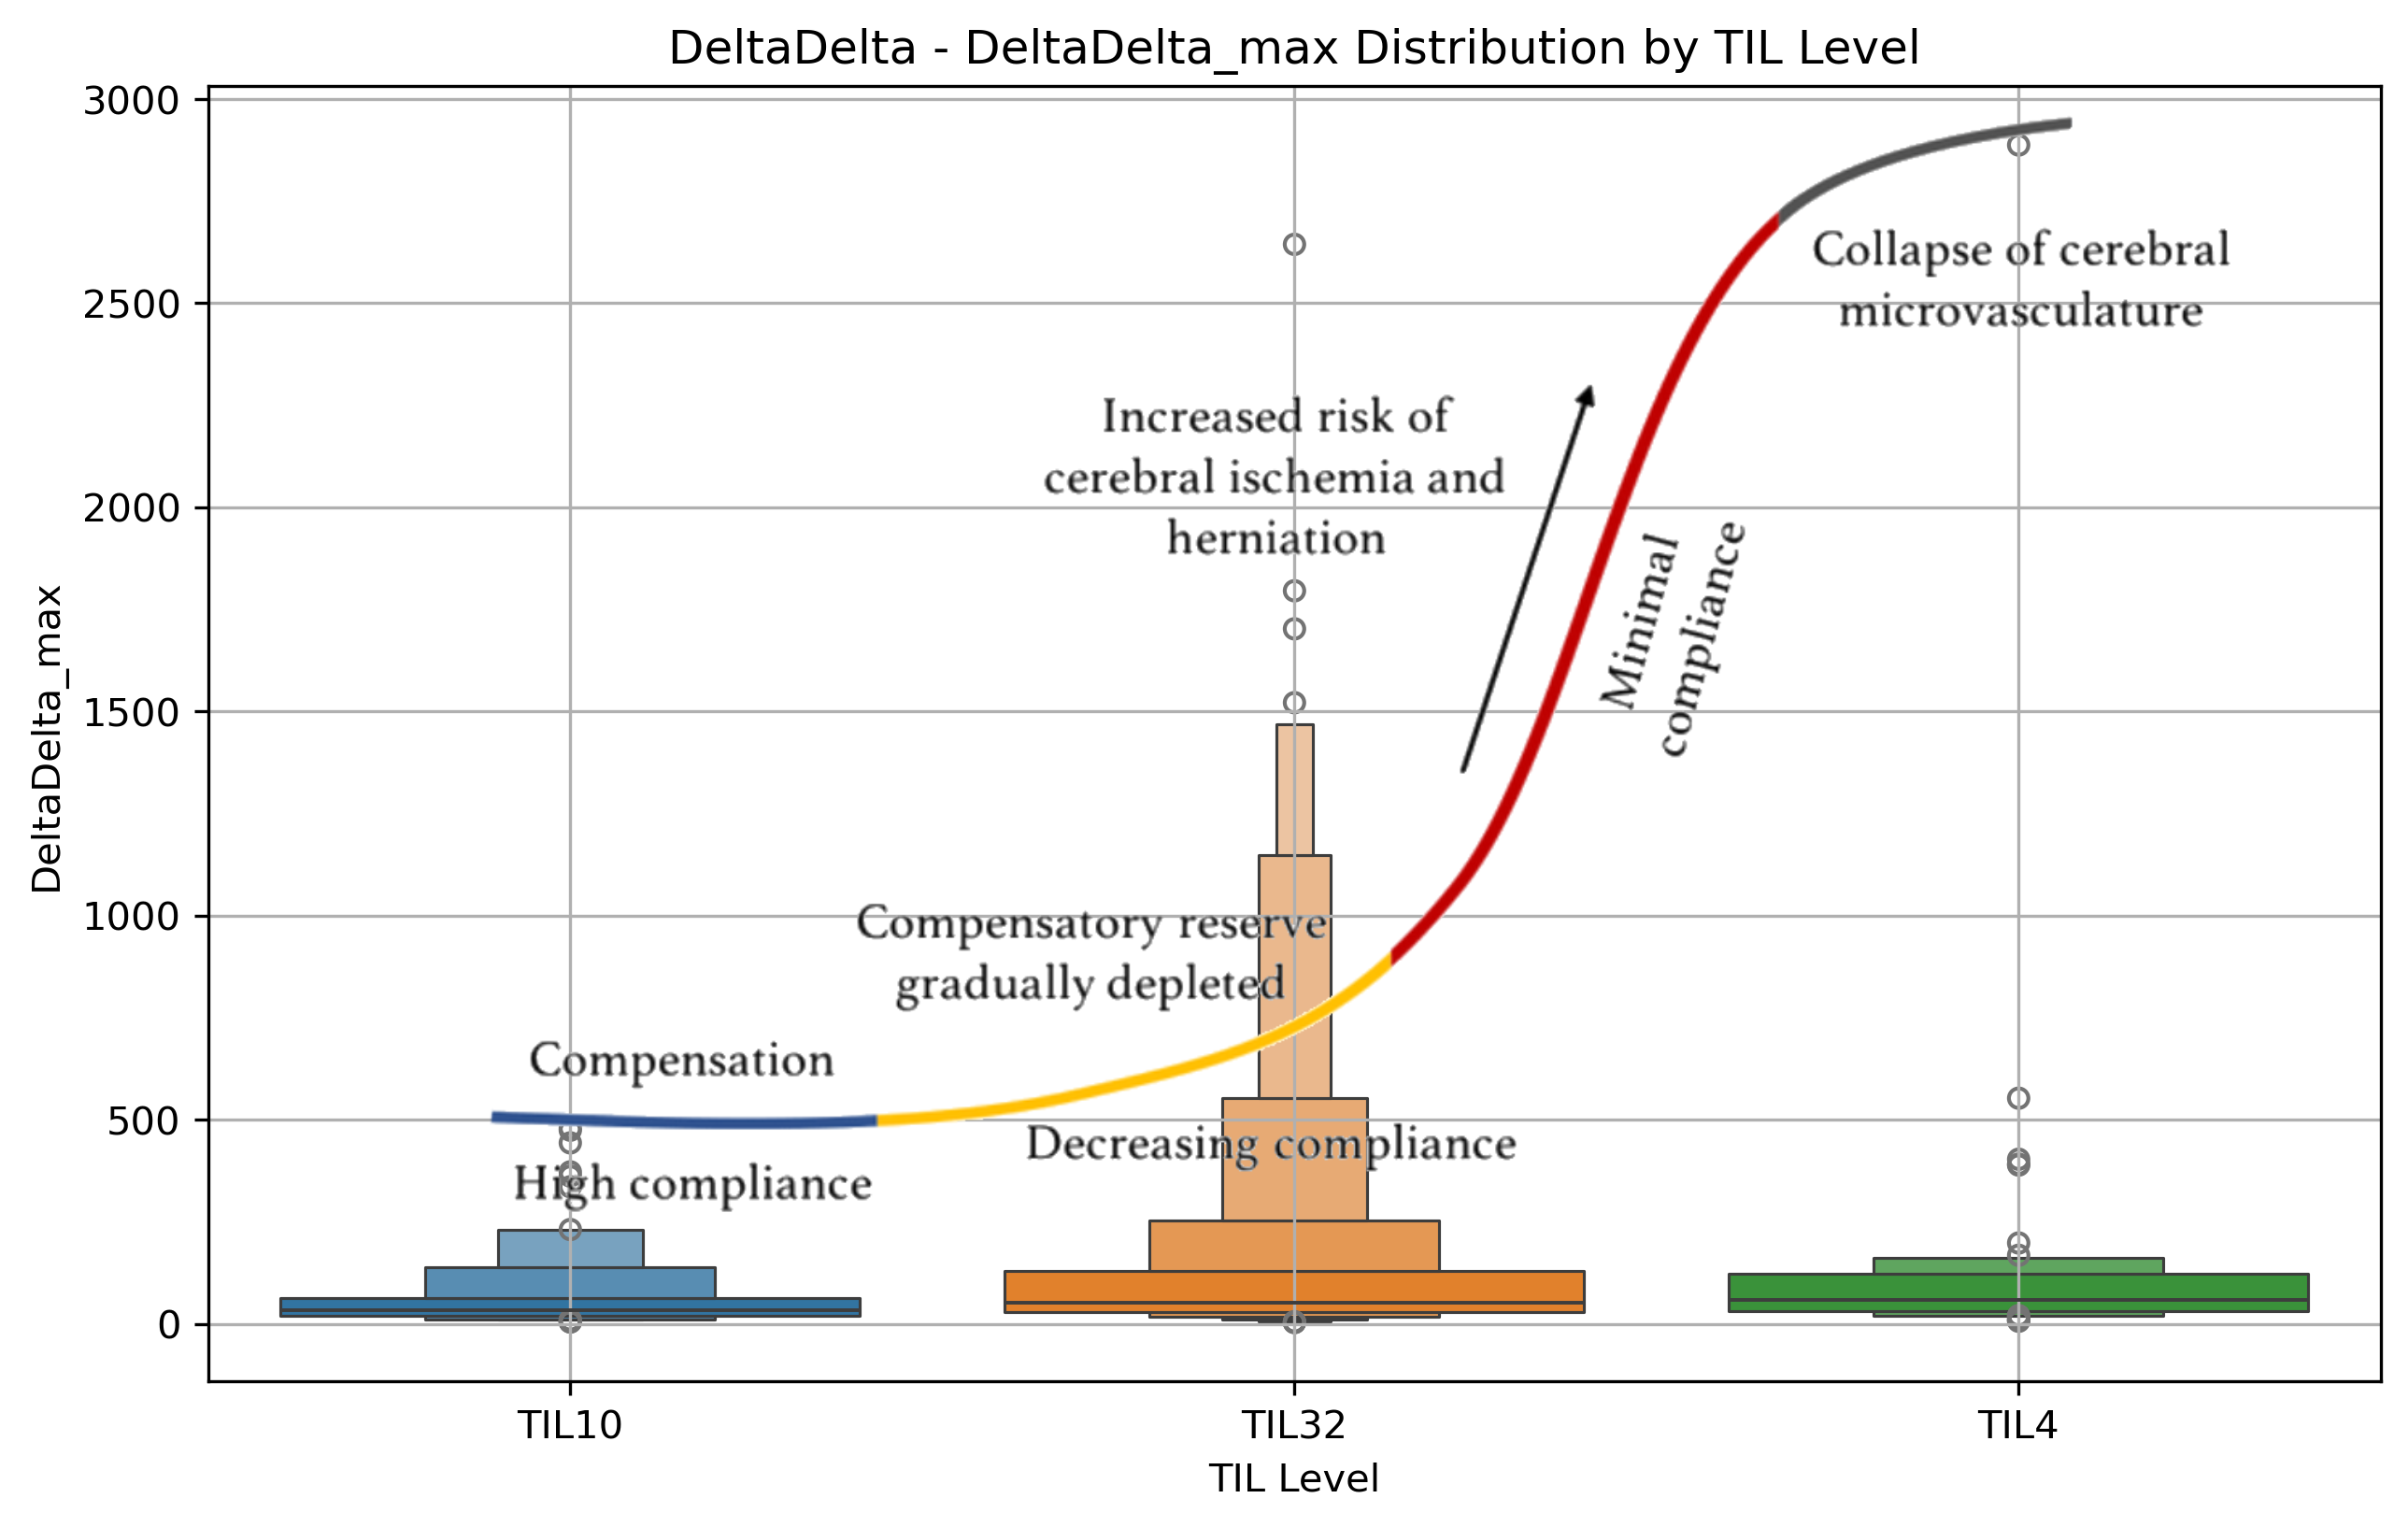
\includegraphics[width=0.8\textwidth]{pictures/fig13_DDTIL.png}
    \caption{DeltaICP/DeltaNa and cerebral compliance} % Add a meaningful caption
    \label{fig:DDTIL} % Add a label for referencing
\end{figure}


\section{Discussion}

\subsection{Machine learning models, what we learned}
As a base model, \textit{Model 1} aims to predict patient outcomes using limited information, primarily focusing on data from the first 24 hours after admission and pre-existing comorbidities. The sodium-related variables are represented by basic statistical features, such as standard deviation. As somewhat expected, this model yielded an AUC of 0.72, indicating a satisfactory level of predictive performance to be used as reference for subsequent models.

In \textit{Model 2}, we investigated the impact of both ICP Dose and Na Dose on patient outcomes. The relationship between ICP Dose and poor prognosis is well-established in the literature\cite{shethIntracranialPressureDose2013}\cite{schonenberg-tuPressureTimeDose2023}\cite{cuccioliniIntracranialPressureClinicians2023a}, and our model supports these findings. However, a noteworthy result is the contribution of Na Dose. While Model 2 incorporates both Na Dose and ICP Dose, some redundancy could be involved as Na Dose in cases of hyponatremia partially contributes to the ICP Dose. Conversely, Na Dose driven by hypernatremia should exhibit a protective effect. One limitation of this model, which may affect bias its performance, is the potential influence of higher ICP doses in patients who underwent WOLST (Withdrawal of Life-Sustaining Treatment), where no further therapeutic interventions to control ICP were applied.
These results appear to validate the integrity of the dataset, providing a solid foundation for progressing to the next model.

With \textit{Model 3} we delved into sodium fluctuations and related ICP fluctuations. 
Severe dysnatremia has long been associated with higher mortality rates while sodium imbalances often arise in TBI patients. Furthermore inappropriate administration or restriction of free water, other comorbidities, treatments, surgery\cite{marshallAssociationSodiumFluctuations2017}\cite{sakrFluctuationsSerumSodium2013}, trauma and acute illnesses\cite{senSodiumVariabilityAssociated2017a} frequently trigger or exacerbate sodium fluctuations. However, emerging evidence\cite{darmonPrognosticConsequencesBorderline2013} indicate that even mild deviations from normal sodium levels or simple fluctuations in sodium values may carry significant clinical implications, especially in the brain injured patient. While this is well documented in subarachnoid hemorrhage \cite{jinAssociationSerumSodium2022}\cite{labibSodiumItsImpact2024}\cite{balesEffectHyponatremiaSodium2016}\cite{topjianGreaterFluctuationsSerum2014}\cite{eaglesSignificanceFluctuationsSerum2019}\cite{haradaImpactHormonalDynamics2022}, the effect on TBI has only recently been explored\cite{harroisVariabilitySerumSodium2021a}. 

In our analysis, even after adjusting for baseline severity, we found that fluctuations in serum sodium and related changes in intracranial pressure (ICP) - also within normal ranges - are associated with 14-day mortality. This reinforces previous findings, such as those reported by Harrois et al.\cite{harroisVariabilitySerumSodium2021a}, confirming that sodium and ICP fluctuations are predictors of mortality in traumatic brain injury (TBI) patients.

Recognizing sodium fluctuations as risk factors associated with mortality could provide new tools in sodium monitoring and management, further evidence to support a type of fluid over the other (hypotonic vs. isotonic) or to define acceptable and individualised sodium fluctuation ranges instead of fixed thresholds. Moreover, identifying sodium fluctuations as an independent risk factor for mortality emphasises the importance of further exploring physiological causes and pathophysiological impact of those fluctuations. 

In our analysis larger fluctuations in DeltaICP/DeltaNa were associated with higher mortality, this could be driven by fluctuations in sodium alone. Rapid changes in sodium levels over a short time may pose a greater risk in patients with disrupted adaptive mechanisms. In the healthy brain, in response to hypertonic conditions in the extracellular space, cells attempt to restore osmotic balance by moving electrolytes and then absorbing organic osmoles, a process that requires time. Sudden shifts in extracellular sodium can lead to intracellular fluid and electrolyte imbalances, resulting in cellular edema or cellular shrinking, particularly in an already injured brain with compromised or slower adaptive mechanisms. An additional challenge lies in understanding how our interventions might affect the unsalvageable brain tissue, raising concerns that some therapies could unintentionally harm the salvageable regions we aim to protect in the first place.

\subsection{Patient Outcomes and Therapy Intensity Levels}
In the subgroup analyses, stratifying patients based on outcome, is still clear as an increasing ICP Dose is found in patients with a poorer prognosis. This is evident in Fig. \ref{fig:ICPdose_outcome}, there is a clear trend of increasing ICP dose as neurological outcomes worsen. Patients with a GCS greater than 8 exhibit the lowest ICP doses, while those with GCS scores below 8 have moderate increases. The highest ICP doses are observed in patients who did not survive, indicating a strong association between elevated ICP doses and mortality. The normalized ICP dose above the threshold increases progressively across the three groups, reflecting the growing difficulty in managing ICP as patient outcomes deteriorate.

Looking together at Fig. \ref{fig:ICPfluctuations_outcome} and Fig. \ref{fig:ICPslope_outcome} key patterns in intracranial pressure (ICP) fluctuations and linear trends relative to neurological outcomes become more evident. In the first one, it is evident that as neurological outcomes worsen, ICP fluctuations, measured by mean crossing rate, show a noticeable decline. This decrease in variability could reflect a progressive exhaustion of cerebral compliance, as the brain becomes less able to accommodate pressure changes, leading to more consistent and sustained elevations in ICP. This loss of fluctuation may indicate that the brain’s adaptive mechanisms are failing. Fig. \ref{fig:ICPslope_outcome} further supports this by showing a clear linear trend: ICP signal slope steadily increases as neurological outcomes worsen. Patients with GCS > 8 exhibit a relatively stable ICP slope, while those with worse outcomes (GCS < 8 and deceased) show a more pronounced upward trend. This suggests a progressive rising trend in ICP over time, further stressing the brain and potentially contributing to worsening outcomes. 

In conclusion, the findings across figures \ref{fig:ICPdose_outcome}, \ref{fig:ICPfluctuations_outcome} and \ref{fig:ICPslope_outcome} present a consistent narrative of progressively increasing ICP burden and worsening neurological outcomes. Those graphs reinforce the importance of early and aggressive ICP dose management with the aim to mitigate secondary brain injury.\\

We then tried to have a quantifiable measure of the intensity of treatments and interventions administered to a brain injured patients with subgroup analysis divided in TIL categories.  In clinical practice, TIL is used to evaluate and categorize the level of therapeutic interventions needed, particularly for managing conditions like elevated ICP. Although our study did not have an objective measure of compliance, a higher TIL suggests more difficulty in managing ICP. Therefore, we can infer that a higher TIL indicates poorer compliance, making TIL a rough proxy for assessing compliance in treatment.
In Fig. \ref{fig:DDTIL}, the mean ICP values are presented for different TILs, revealing an intriguing pattern. The intermediate TIL group demonstrates a notably higher mean ICP compared to the most severe category (TIL 4 or extreme TIL). This counterintuitive observation could suggest that at higher TIL levels aggressive therapeutic interventions (e.g., hyperosmolar therapy or decompressive craniectomy) are more frequently employed to manage ICP,  limiting further increases in pressure. In contrast, at intermediate TILs, ICP may be more difficult to control, leading to higher values. 
\textcolor{red}{INSERIRE GRAFICO ICP DOSE E TIL PER VEDERE SE MIGLIORA: CIOE LA DOSE ICP IN TIL 2 è PIU BASSA CHE IN TIL 4 -> RAFFORZEREBBE IL CONCETTO DELLA ICP DOSE!}
Fig. \ref{fig:DDTIL} illustrates how the DeltaICP/DeltaNa ratio changes across TIL levels. In patients with lower TILs the brain seems able to compensate for increases in ICP, if any occurs at all. As the TIL increases, this could represent a gradual depletion of compensatory reserves and a significant rise in ICP, accompanied by an increased risk of cerebral ischemia and herniation. By the time patients reach the highest TIL level (TIL 4), cerebral compliance is nearly depleted, suggesting that most compensatory mechanisms have been exhausted. At this stage, ICP has likely reached its maximum plateau, which accounts for the reduced variability in fluctuations observed at the extreme TIL level. Since DeltaICP/DeltaNa is a ratio of relative changes, as these fluctuations diminish and ICP can no longer vary significantly due to this plateau, the DeltaICP/DeltaNa ratio becomes less meaningful in reflecting further dynamic changes. It’s also likely that patients who either died or had poor neurological outcomes at 14 days experienced a wider range of sodium concentrations due to treatments such as hypertonic saline, this could further explain those minimal fluctuations occurring at consistently elevated levels of sodium (as part of the therapeutic approach) and ICP (resulting from exhausted cerebral compliance).
At the opposite, the DeltaICP/DeltaNa ratio of the intermediate TILs suggests that larger fluctuations in serum sodium are associated with the need for higher therapy intensity levels, raising the possibility that acute sodium variations may partially explain the relationship between DeltaICP/DeltaNa and patient outcomes.\\

\textcolor{red}{FARE GRAFICO DOVE PER TIL MOSTRIAMO MORTI E VIVI? COSI SPUNTO PER QUANTO LA NOSTRA TP AGGRESSIVA -> TIL 4 I VIVI SONO MOLTISSIMI MA LO STATO NEUROLOGICO È PESSIMO, SONO I NOSTRI TRATTAMENTI AGGRESSIVI TROPPO TARDIVI? ES CRANIECTOMIA DECOMPRESSSIVA? SALVIAMO L'ORGANISMO MA NON IL CERVELLO}
\\


%parlando di TIL, specificare come le distribuzioni dei nostri pazienti siano sovrapponibili con quelle di altri studi: es SYANPSE-ICU

\subsection{Limitations}
This is a retrospective study, and as such, it carries the inherent limitations associated with this type of research.

We did not assess neurological outcomes nor the Glasgow Outcome Coma Scale was available in our database. This limitation should be addressed in future studies investigating sodium fluctuations in TBI patients.

We didn't assessed the impact of intravenous fluid administration on sodium variability, as it was challenging to extract detailed information regarding the specific types of hypertonic saline\cite{holdenHypertonicSalineUse2023a} used for osmolar therapy.
For similar reasons, we didn't assessed the impact of diabete insipidus through desmopressin administration, as considering it alone as a surrogate marker woulnd't have been enough to diagnose DI or to discriminate with other brain-related plasma sodium disorders (SIADH or CSW). 

Although we adjusted for TIL, serum sodium fluctuations may still be a reflection of overall illness severity. Nevertheless, dysnatremias remain a known risk factor and should be incorporated into future predictive models for mortality in TBI patients, including fluctuations within normal limits, rather than dismissed as a mere consequence of disease severity.

Additional limitations in the subanalysis of patients within TIL therapy categories, beyond the already mentioned hypertonic saline, include missing data on decompressive craniectomy\cite{kimRecentUpdatesControversies2023a} and other interventions that are difficult to associate with specific treatment goals. For instance, it’s unclear whether vasopressors were used to manage elevated ICP or for other hemodynamic purposes, further complicating the analysis.

Lastly, patients who died within the first three days were excluded, which may limit the generalizability of our results.


\section{Conclusion}
While doses of potassium, glucose, and water are routinely adjusted, sodium is typically administered at standard concentrations as long as serum levels remain within an acceptable or desired range. This is common practice in many ICU patients and is well tolerated in most cases. However, for the peculiar brain injured patient, the sodium content may not align with the intravascular volume or neuroendocrine status, leading to impaired sodium homeostasis. 
Our findings highlight the importance of monitoring both sodium and ICP fluctuations in critical care settings, particularly in neurocritical care patients. Our work suggests that even within clinically acceptable ranges, significant sodium variability is linked to poorer outcomes.

The DeltaICP/DeltaNa ratio, which reflects the relationship between sodium and ICP fluctuations, shows that larger sodium fluctuations are associated with more aggressive therapeutic interventions and worse neurological outcomes. This further supports the idea that sodium fluctuations, rather than absolute levels, may play a critical role in patient prognosis. As cerebral compliance becomes increasingly impaired, as seen in higher Therapy Intensity Levels (TILs), sodium variability could exacerbate the risk of secondary brain injury due to osmotic shifts and the body’s diminishing ability to regulate ICP.

Given these findings, it may be prudent to consider shifting the focus toward minimizing sodium fluctuations and maintaining osmolality stability rather than solely aiming to keep serum sodium levels within a “normal” range. By reducing the dynamic shifts in sodium and ensuring a stable trajectory, we could potentially mitigate the risk of further cerebral damage, particularly in patients with compromised brain compliance. This underscores the need for a more individualized approach to sodium management in the ICU, where therapy intensity and the patient’s fluctuating physiological state should inform fluid and electrolyte administration.




